\documentclass{article}
\usepackage[utf8]{inputenc}

\usepackage{url}
\usepackage[numbers]{natbib}
\usepackage{indentfirst}
\usepackage{graphicx}
\usepackage{geometry}
\usepackage{listings}
\usepackage{float}

\begin{document}

\title{Blockchain based investment cooperative application}
\author{\IEEEauthorblockN{Mubarak Mikail, Sam Seneza}\\
\IEEEauthorblockA{\textit{College of Engineering} \\
\textit{Carnegie Mellon University Africa}\\
Kigali, Rwanda \\
\{mmikail, sseneza\}@andrew.cmu.edu}
}
\date{February 2020}

\maketitle

\section{Introduction}
The number and size of cooperatives around keeps increasing day-by-day which also goes with the rise in the amount of money that is being contributed. Book-keeping, safekeeping, and the security of the circulation of money gets more and more tedious. This paper looks into how these processes can be made simpler and more secure with Blockchain technology which is simply a data structure used for storing data and more formally which can be regarded as an open distributed ledger which stores transactional data in a way that is permanent and persistent, that is they cannot be edited or modified once they are on the blockchain. Every transaction that take place on the blockchain is known to all parties involved, hence there is no form of secrecy involved as everything is made public.

\subsection{Background of the project}
Cooperative contribution involves a group of people coming together to pull some money together on either a monthly, quarterly or yearly basis and at the end of that period, one person takes all the money, another person in the group takes the one for the next period and it goes on like that until everyone gets their fair share before the cycle comes back to continuity. This functioning cooperative is set in order to raise funds to help its members to get increased access to monetary resources without the hassle of requesting loans from banks. This implies that members can also request for loans from the cooperative and would have to pay back after a certain period of time with some additional charges.

Cooperative saving and credit institutions can be traced to the 19th century especially in Germany where there was a credit cooperative for minor artisans and the urban middle classes \cite{galor2018saving}. These types of cooperatives are basically put in place to avoid the difficulties of obtaining credit from a bank. The cooperative members help each other to prevent poverty with mutual aid and self-reliance. Members are encouraged to contribute money, and this money enables them to receive loans from their accumulated savings for various reasons. The benefits of cooperatives are not only reaped by the loan seekers, they are reaped by everyone because whenever one of the members take a loan, they repay the money with some interest that can be shared among the cooperative members. Cooperative contribution can in some ways also be a safeguard to money of the parties involved since the cumulative amount can be shielded in advantage over time. \cite{galor2018saving}

In cases where a member gets money from the cooperative, the factors influencing repayment vary depending on interest rates, the duration of loans, personal sources of income, and much more \cite{papias2009repayment}. This may raise the uncertainty of member’s money safety. Bookkeeping of the cooperative’s money may be exasperating, and ways to misuse the money may arise from the process.

\subsection{Problem Statement}
Cooperatives are operated in different ways, however for our project we drill down on the cooperative approach in general i.e., members contribute together and then choose one of them to take all the money (or a certain amount agreed on by all members) in the cooperative. This person may use the money in a variety of their own projects and may be expected to pay back after a certain period of time with a set interest depending on the agreement. This cooperative money in some cases may be highly controlled by the cooperative president \cite{nilsson2013cooperative}.

Digging deeper into the current cooperative functioning system, a cooperative president who may have some superior control over the cooperative money may decide to misuse these funds. A person may get to be selected to take the money cyclically with some bias. A person who takes/borrows the money may, with little or no difficulties, erase the traces that they are in a temporal possession of the money. These kinds of problems do occur especially with the non-transparent decision-making process within cooperatives, limited managerial or leadership capacities by some members, and external help in connection with the cooperative's development \cite{rca001}. This problem could be summarized generally as the misuse of cooperative funds as this non-transparency mostly suggests. However, a digital decentralized solution could be employed as a smart way to mitigate these kinds of problems.

These problems could be addressed with the introduction of a distributed ledger technology i.e., a blockchain in order to address the problem of one privileged member to misuse the funds as each and every transaction would be stored permanently and irreversibly in the system. This would make the exchange of information regarding the movement of money easy and with more clarity \cite{rodrigues2019evaluating}. In addition to this, the problems regarding the possibility of bias in the selection of who to receive the money at a certain period would be eliminated with a digital system that would purely select randomly which of the members is to receive the money.

\subsection{Area of Focus}
A functioning cooperative is set up in order to raise funds to help its members to get increased and fast access to monetary resources without the bottlenecks involved in requesting loans from banks. This cooperative system is designed and agreed on by cooperative members that are willing to join and due to this fact, some people may think that when choosing who should take the money there is some bias (which may also be true in some cases). And if this can happen, it suggests that the system may need some improvements. What if there was a digital system to randomly select one person, that person then becomes the one assigned to take the money for their use, and then that system removes that person from the possibility to be randomly selected before the cycle restarts. In other words, once a person is selected, they are removed from the choices within the same cycle, but they are to be brought again after the cycle ends hence ensuring that no person is selected to get the money twice within one cycle.

In the current traditional method of managing cooperative activities, a third party watcher may have to be involved in order to ensure smooth and trusted operations \cite{nair2018blockchain}. An improvement here would be bringing in blockchain to record cooperative members’ contributions with a specialty of being publicly verifiable \cite{nair2018blockchain}. And in addition to that, an unbiased algorithm to select who should take the money at a certain point in the cycle would be incorporated into the technology therefore improving the reliability of the cooperative functioning. 

\section{Literature Review}
A cooperative is basically a firm that is set up by a group of people to serve for collective benefit. They contribute monetary resources together so that they so to share and meet specific target objectives. Generally within cooperatives, people can also get loans usually at smaller interest rates compared to regular financial situations. A cooperative can also be referred to as a business organization with limited liability where each shareholder has on vote regardless of the shares they own \cite{credo22393191}. The stress of a cooperative functions are expressed as an organization that is operated for the benefits of the people using its services that may be mostly its members \cite{credo17700186}.

Cooperative work's efficiency may be improved by solving extensively some of its current major problems and some of those current problems are listed below:
\begin{enumerate}
    \item The capacity of cooperative leadership and management.
    \item Lack of democratic control by the members.
    \item Third party involvement which could lead to collusion, theft and fraud.
\end{enumerate} 

These problems stated above are imperceptibly contrary i.e., are equivalent with the tendency of misusing as discussed in the statement of the specific problem. 

A recent study of 450 cooperatives in Tanzania and Sri Lanka reports that cooperatives lack access to loan finance to help them expand their business. 
 
“Equality is one of major guiding values of cooperatives. An open and voluntary membership is one of the principles to which cooperatives hold dear. Cooperative enterprises prefer to have a “one member, one vote” system, which ensures that decision making powers are equally distributed amongst the members . Cooperatives are people-centric enterprises, hence they end to focus on the needs of their members and of the communities in which they operate, rather than on financial returns alone.” \cite{un_issues} This is related to the second problem stated above.

Regarding the capacity of the cooperative leadership and management, and the lack of democratic control by the members of a cooperative can lead to the doom of their endeavors. Research has found that the growth of these kinds of organizations may be facilitated by relying on blockchain technology as their source of distributed governance or control. \cite{mannan2018fostering}

Another research has also spotted a potential means to the improvement of cooperative leadership and management. This specifically is the transparent and available bookkeeping where it was stated that the blockchain technology can be of great importance in improving the bookkeeping methods of Kenyan cooperatives basically because all activities would be transparent and available to everyone anytime. \cite{mitch_national}

A proposal in a research suggests a blockchain federated intermediary architecture in order to help everyday cooperation activities. This proposal goes a step further showing the benefits that could be witnessed by a number of cooperatives with heterogeneous information i.e., separated information if all cooperative chains' information was now made easy to be traversed. \cite{ieee_s8637578} 

Research has shown that blockchain can be used as a data sharing platform for cooperative purposes while ensuring its overall security, and also most importantly ensuring its traceability towards the satisfaction off human needs in cooperatives. \cite{alma991019580288704436, proquest2282979983} 

Primarily, we are trying to solve this possibility of funds misuse as specified above by ensuring transparent cooperative leadership and transactions. Blockchain can help us with tackling the challenges of lack of democratic control among the members and third party involvement in the cooperative activities which usually have detrimental effects on the society.
Not a lot of work has been done prior to this time in this regard though research has highlighted and addressed most of these problems and how they can be resolved by a blockhain network. This implies that transparency in everyday cooperative activities could be fortified towards the mitigation of the problem of misusing funds in cooperatives.

This new system is trying to address these problems stated above, as from empirical research were they found. This system will incorporate the blockchain technology in everyday transactions of cooperatives, set out from contribution to sharing, returning the cooperative money with collective clarity.

\section{Proposed Solution}
The goal of this solution is to make easy the cooperative contribution currently done manually by people. Our proposed solution is a decentralized application that is going to employ a DLT (Distributed Ledger Technology) which is a distributed non-repudiatory way in keeping track of the amount of money each member of the group is contributing to the wallet i.e., contributions should be recorded trace by trace permanently. Unlike current systems where there are issues when it comes to determining who gets paid for each period as people might not be very comfortable with them not getting their share early in the contribution stages. 

An algorithm will be employed to select recipients of the general contribution for each period, this will bring some trust to this group. The algorithm will involve assigning unique ids to each member of the cooperative such that at the end of each period that is at the time of collections, a unique id will be selected from that pool by the computer and the owner of that id gets the contributions for that period, this id is then taken out of the pool. This will be iterated every period end.

This solution can be extended to investments in other cryptocurrencies and other commodities in the near future. An individual can also choose to use it to save money over a period. The DLT is there to show the amount everyone is contributing, there is fairness and trust as everyone involved will have access to this data. There are certain challenges that might be associated with this solution, however we will look at how to mitigate these challenges.

\begin{figure}[h!]
\centering
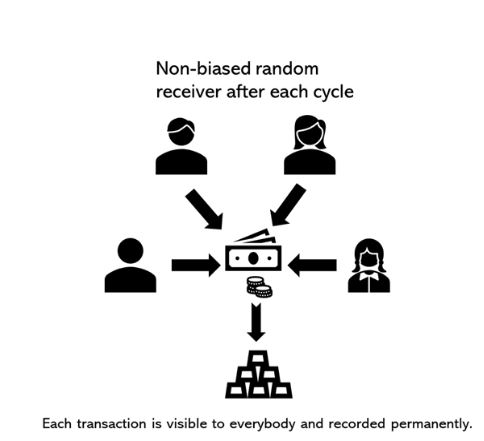
\includegraphics[scale=1.0]{cop}
\caption{Overview of the proposed solution}
\label{fig:central}
\end{figure}



\section{Methodology}
This solution is going to be implemented in 2 main parts:
\begin{enumerate}
    \item General algorithm for the decentralized application
    \item Algorithm for selecting which of the members gets paid at the end of the period.
\end{enumerate}

The selection of who gets paid has been discussed in the previous section on proposed solution & algorithm. Here, we will talk more about a general algorithm for implementing our application. Much of the coding of our smart contract is going to be done in Solidity. We will start by creating a contract in solidity that will represent the main contract between any cooperative group. This will have certain features like members and each member will have a means of identification on the blockchain which is going to be their address. This will be generated off the Ethereum Blockchain.
Some of the deliverables we hope to achieve at the end of this project are:
\begin{itemize}
    \item A working decentralized application.
    \item A group of people should be able to come together and form a cooperative on this App.
    \item They should also be able to send money to a particular address.
    \item All transactions to this address must be visible to everyone in the group especially.
    \item We aim to implement this solution as a web application.
\end{itemize}

\subsection{Tools and Datasets}
This solution is going to ride on Ethereum as the main blockchain technology. Most decentralized applications run on ethereum. Ethereum has two main components: Smart contracts and DLT, they will be very important in this implementation. On Ethereum, applications that can control digital value and are accessible from any part of the world can be implemented. Solidity and JavaScript will be used to build the application. Remix IDE will be used to write and compile our Solidity program.

\begin{figure}[H]
\centering
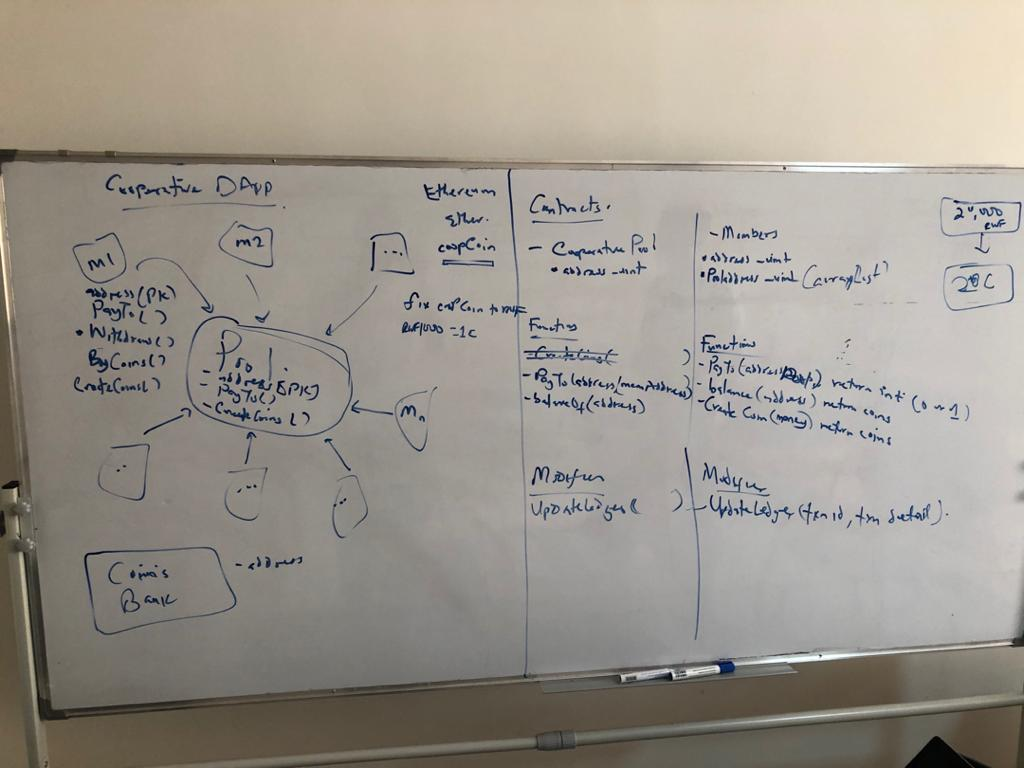
\includegraphics[scale=0.4]{design}
\caption{Blackboard sketch of the design}
\label{fig:dessign}
\end{figure}

\begin{figure}[H]
\centering
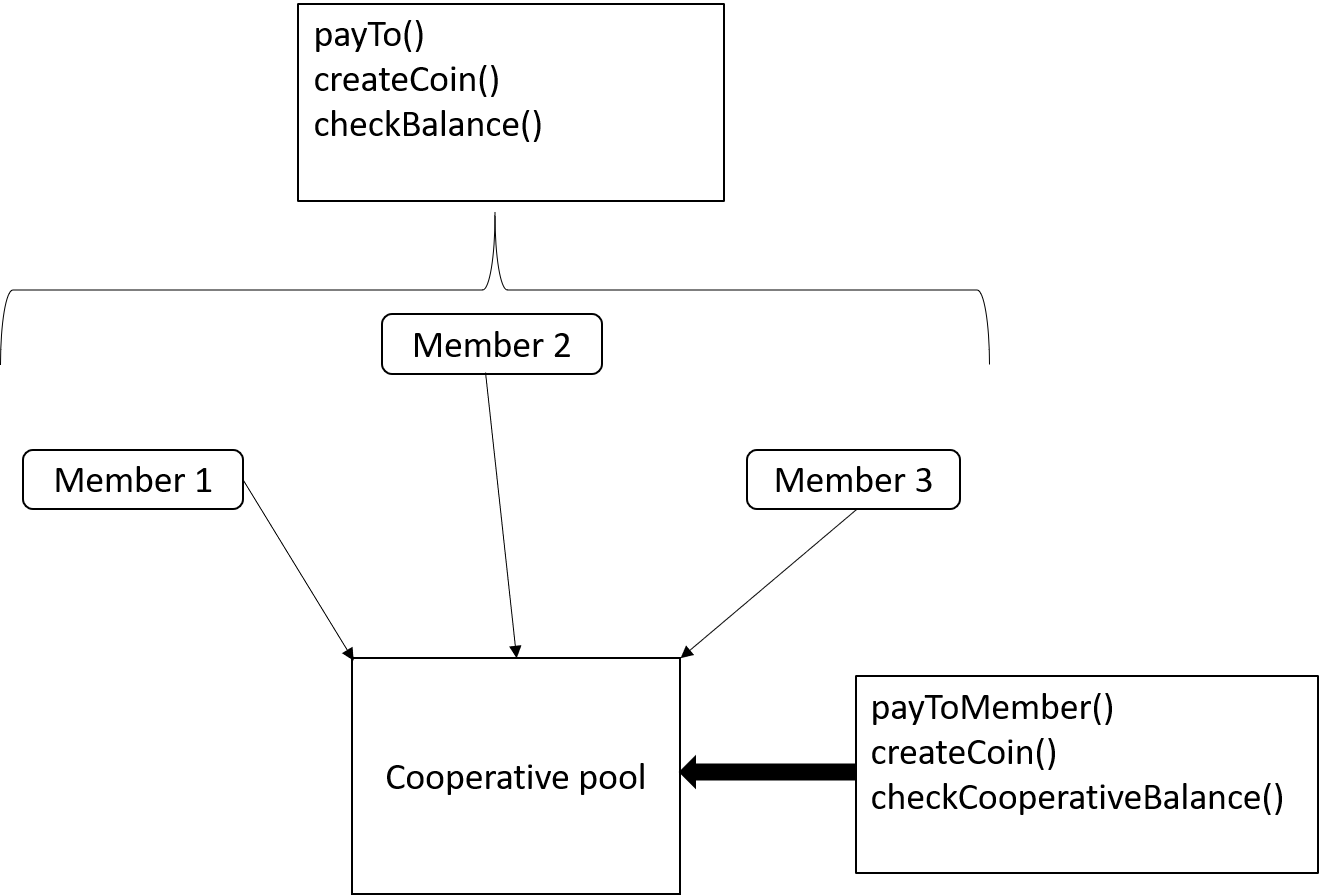
\includegraphics[scale=0.4]{KeyFunct.png}
\caption{Illustration of key functionalities of the application}
\label{fig:dessign}
\end{figure}

\section{Implementation}
The blackboard sketch of our design is shown in Fig. 2. We are modelling our design in a way such that we have basically two(2) main contracts. A member contract where we are trying to abstract away all the details and functions of members in the cooperative. The other contract is the Cooperative pool contract, here we have the details of the pool where we them members will be transferring their contributions to. In the cooperative pool contract we also have functions that we want the pool to be able to perform. 



\section{Results and Discussion}
Some of the results we wish to achieve from this implementation include:
\begin{itemize}
    \item Successfully set up a contract for members
    \item Successfully set up a cooperative pool contract
    \item Ability to make transfers between these two contracts
    \item Ability to see the balance left on these contracts
\end{itemize}


\section{Conclusion}

\bibliographystyle{ieeetr}
\bibliography{references}
\end{document}
